\documentclass[aspectratio=169,11pt]{beamer}

\usetheme{Madrid}
\usecolortheme{default}
\usefonttheme{professionalfonts}
\setbeamertemplate{navigation symbols}{}
\setbeamertemplate{footline}[frame number]

\usepackage{amsmath, amssymb, booktabs, graphicx}
\graphicspath{{../../assets/figures/}{assets/figures/}}

\title{Wage Determination and Returns to Skill}
\subtitle{Labor I --- Week 5}
\author{Teaching deck draft}
\date{}

\begin{document}

\begin{frame}
  \titlepage
\end{frame}

\begin{frame}{Central question and motivation}
\begin{itemize}
    \item Week 5 asks how markets translate accumulated skill into observed wages.
    \item A schooling premium can bundle productivity, selection, sorting, amenities, and rents.
    \item The recurring question is not just ``is the effect causal?'' but ``which return object are we estimating?''
\end{itemize}
\end{frame}

\begin{frame}{Week 4 to Week 5 bridge}
\begin{itemize}
    \item Week 4 treated skill as an accumulated state variable.
    \item Week 5 treats wages as equilibrium outcomes that price that state only imperfectly.
    \item We therefore move from human-capital accumulation to wage measurement, identification, and sorting.
\end{itemize}
\end{frame}

\begin{frame}{Mincer benchmark}
\[
\log w_i = \alpha + \rho s_i + \beta_1 x_i + \beta_2 x_i^2 + \varepsilon_i
\]

\begin{itemize}
    \item Useful benchmark decomposition of wage differences by schooling and experience.
    \item \(\rho\) is descriptive unless stronger assumptions make it causal.
    \item Wage returns are not the same as productivity returns, especially once hours and job assignment matter.
\end{itemize}
\end{frame}

\begin{frame}{Stylized Mincer profiles}
\begin{center}
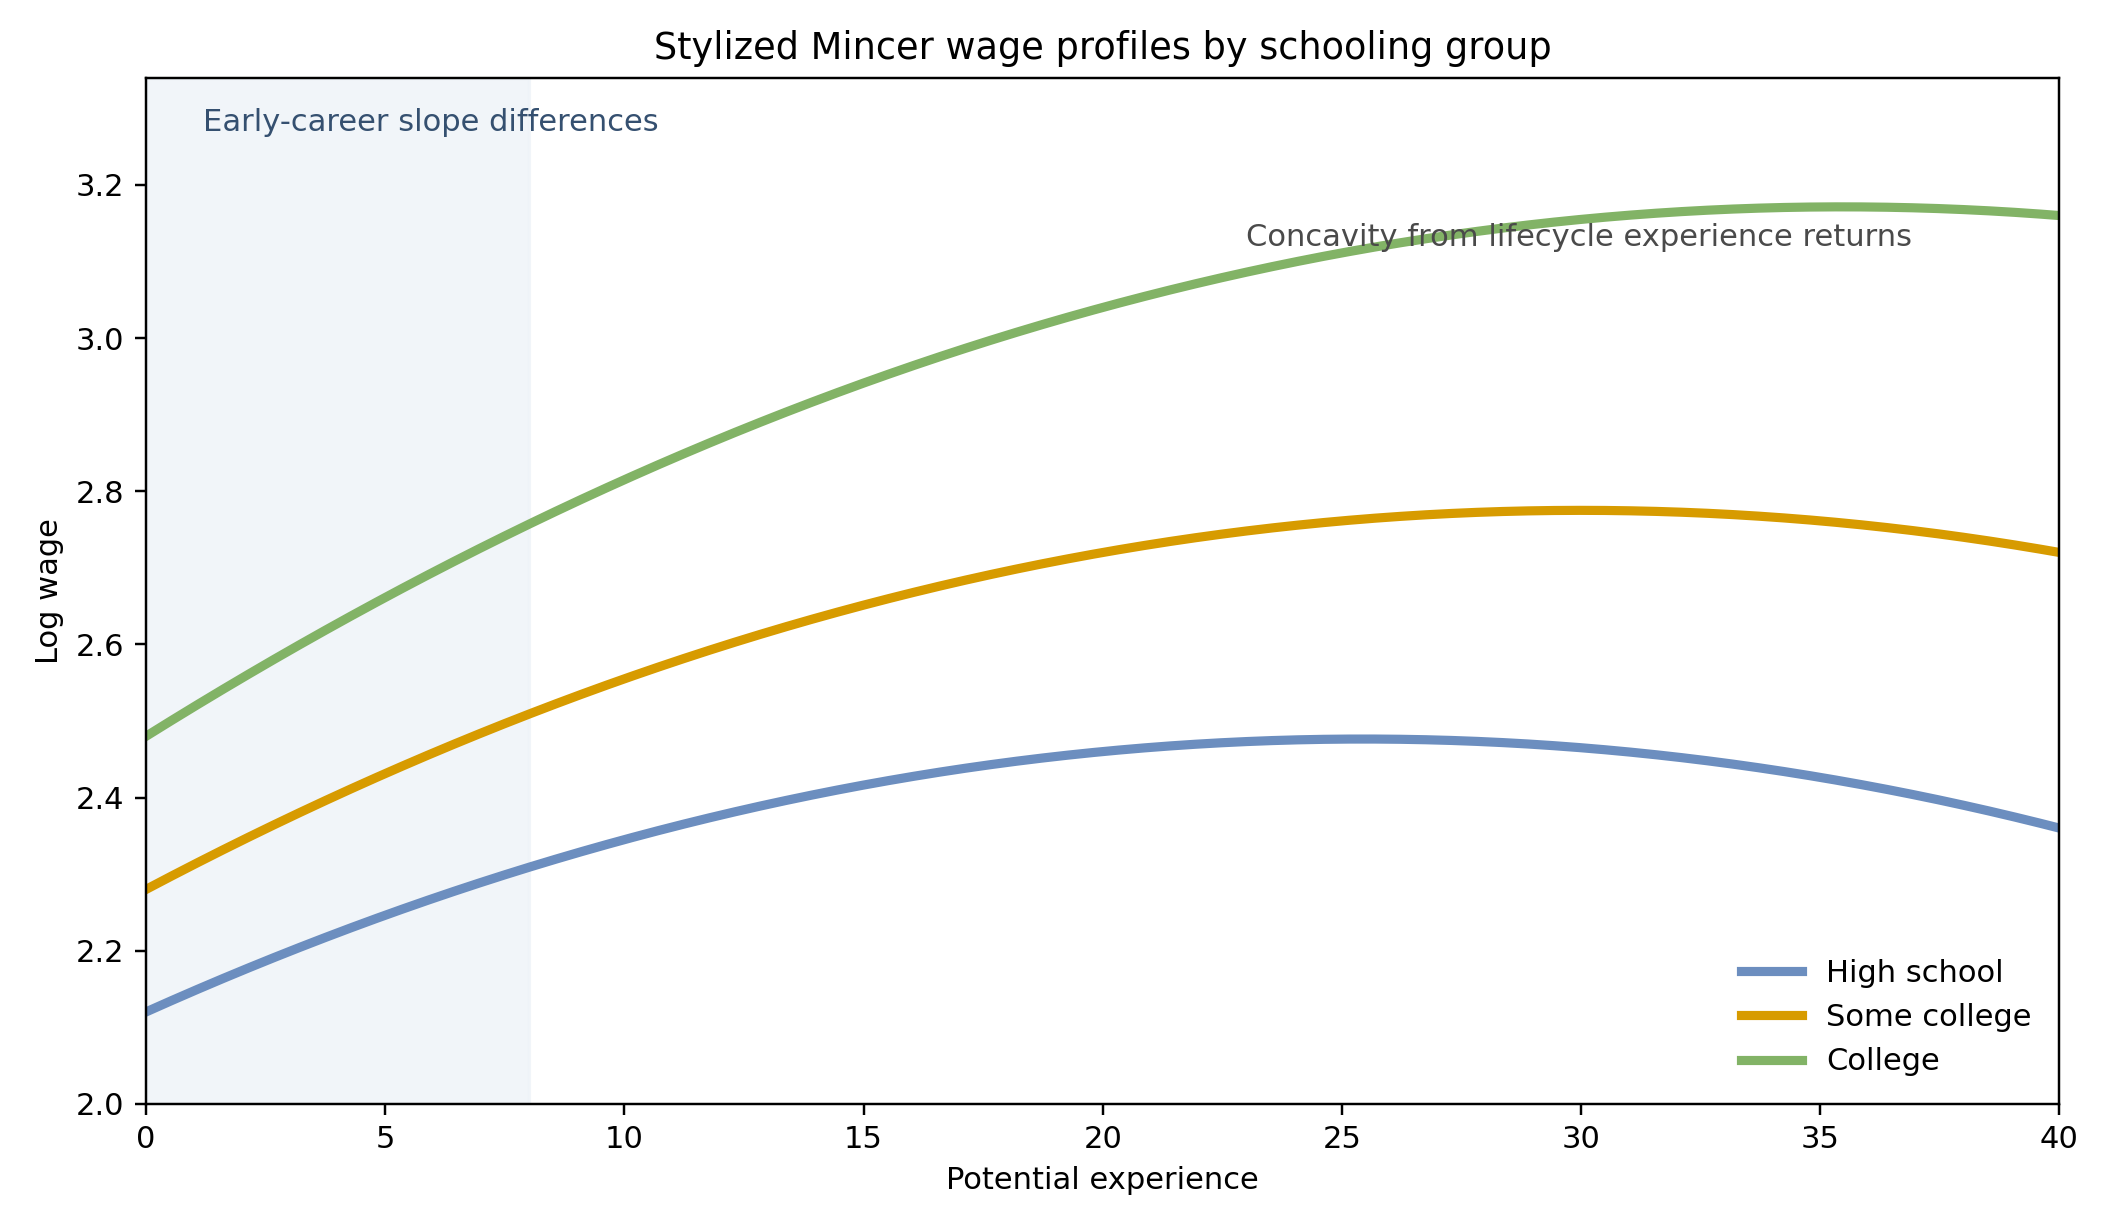
\includegraphics[height=0.74\textheight,keepaspectratio]{05-mincer-wage-profiles.png}
\end{center}
\end{frame}

\begin{frame}{Selection and heterogeneous gains}
\[
Y_i(s) = \mu_i + g_i(s)
\]

\begin{itemize}
    \item Selection is not only ability bias in levels.
    \item Comparative advantage means workers sort on gains as well as on baseline productivity.
    \item OLS, IV, and structural approaches answer different questions once \(g_i(s)\) varies across people.
\end{itemize}
\end{frame}

\begin{frame}{What does IV estimate?}
\[
\beta^{IV}
=
E\left[
\frac{Y_i(1)-Y_i(0)}{S_i(1)-S_i(0)}
\middle|
S_i(1) > S_i(0)
\right]
\]

\begin{itemize}
    \item Compulsory-schooling IV identifies a local return for the margin shifted by the policy.
    \item Oreopoulos is useful because the first stage is economically meaningful.
    \item Stephens and Yang remind us that familiar instruments can still be trend-sensitive.
\end{itemize}
\end{frame}

\begin{frame}{OLS versus IV / LATE}
\begin{center}
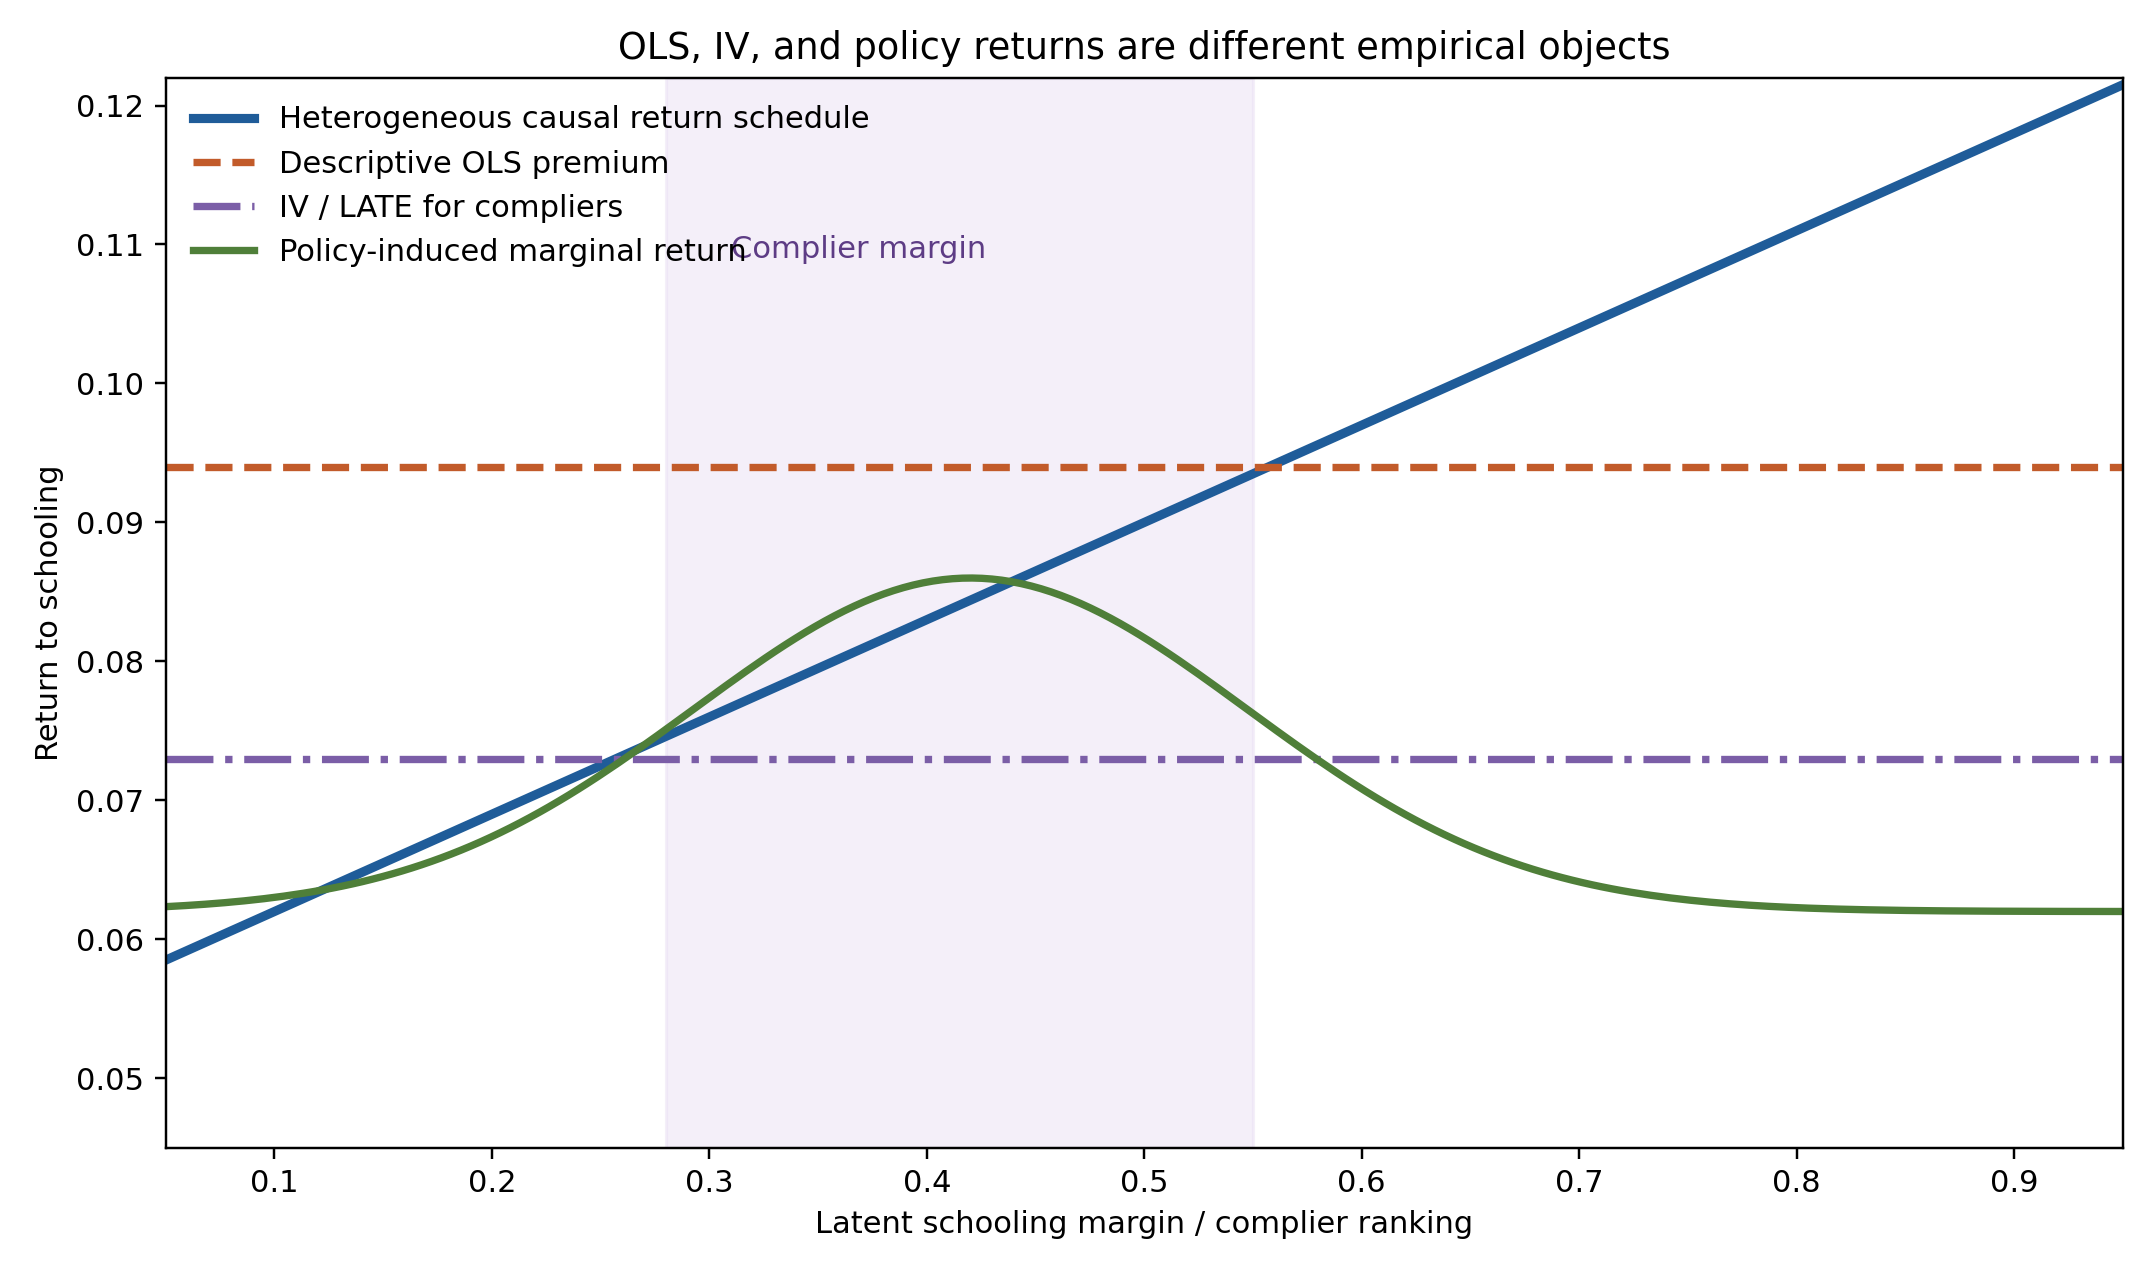
\includegraphics[height=0.74\textheight,keepaspectratio]{05-ols-iv-late-objects.png}
\end{center}
\end{frame}

\begin{frame}{Parameter map for returns-to-schooling research}
\small
\begin{tabular}{p{0.20\linewidth} p{0.23\linewidth} p{0.24\linewidth} p{0.24\linewidth}}
\toprule
Object & Design & What it measures & Main threat \\
\midrule
OLS premium & Mincer regression & Conditional schooling-wage association & Selection and sorting \\
ATE & Strong structure / experiment & Mean causal gain & External validity \\
LATE & Compulsory-schooling IV & Return for compliers & Margin-specific interpretation \\
Marginal policy effect & LIV / structural & Policy-induced local gain & Support and functional form \\
Firm-mediated return & Matched worker-firm data & Share of premium via better firms & Firm effects bundle rents and selection \\
\bottomrule
\end{tabular}
\end{frame}

\begin{frame}{Wages are also shaped by firms and places}
\[
\log w_{it} = \alpha_i + \psi_{j(i,t)} + x_{it}'\beta + \varepsilon_{it}
\]

\begin{itemize}
    \item Wage dispersion can reflect worker effects, firm premia, and market assignment.
    \item Education may raise wages partly by improving access to higher-paying firms or cities.
    \item This is why Week 5 is also the bridge into inequality and mobility work.
\end{itemize}
\end{frame}

\begin{frame}{Worker-firm sorting schematic}
\begin{center}
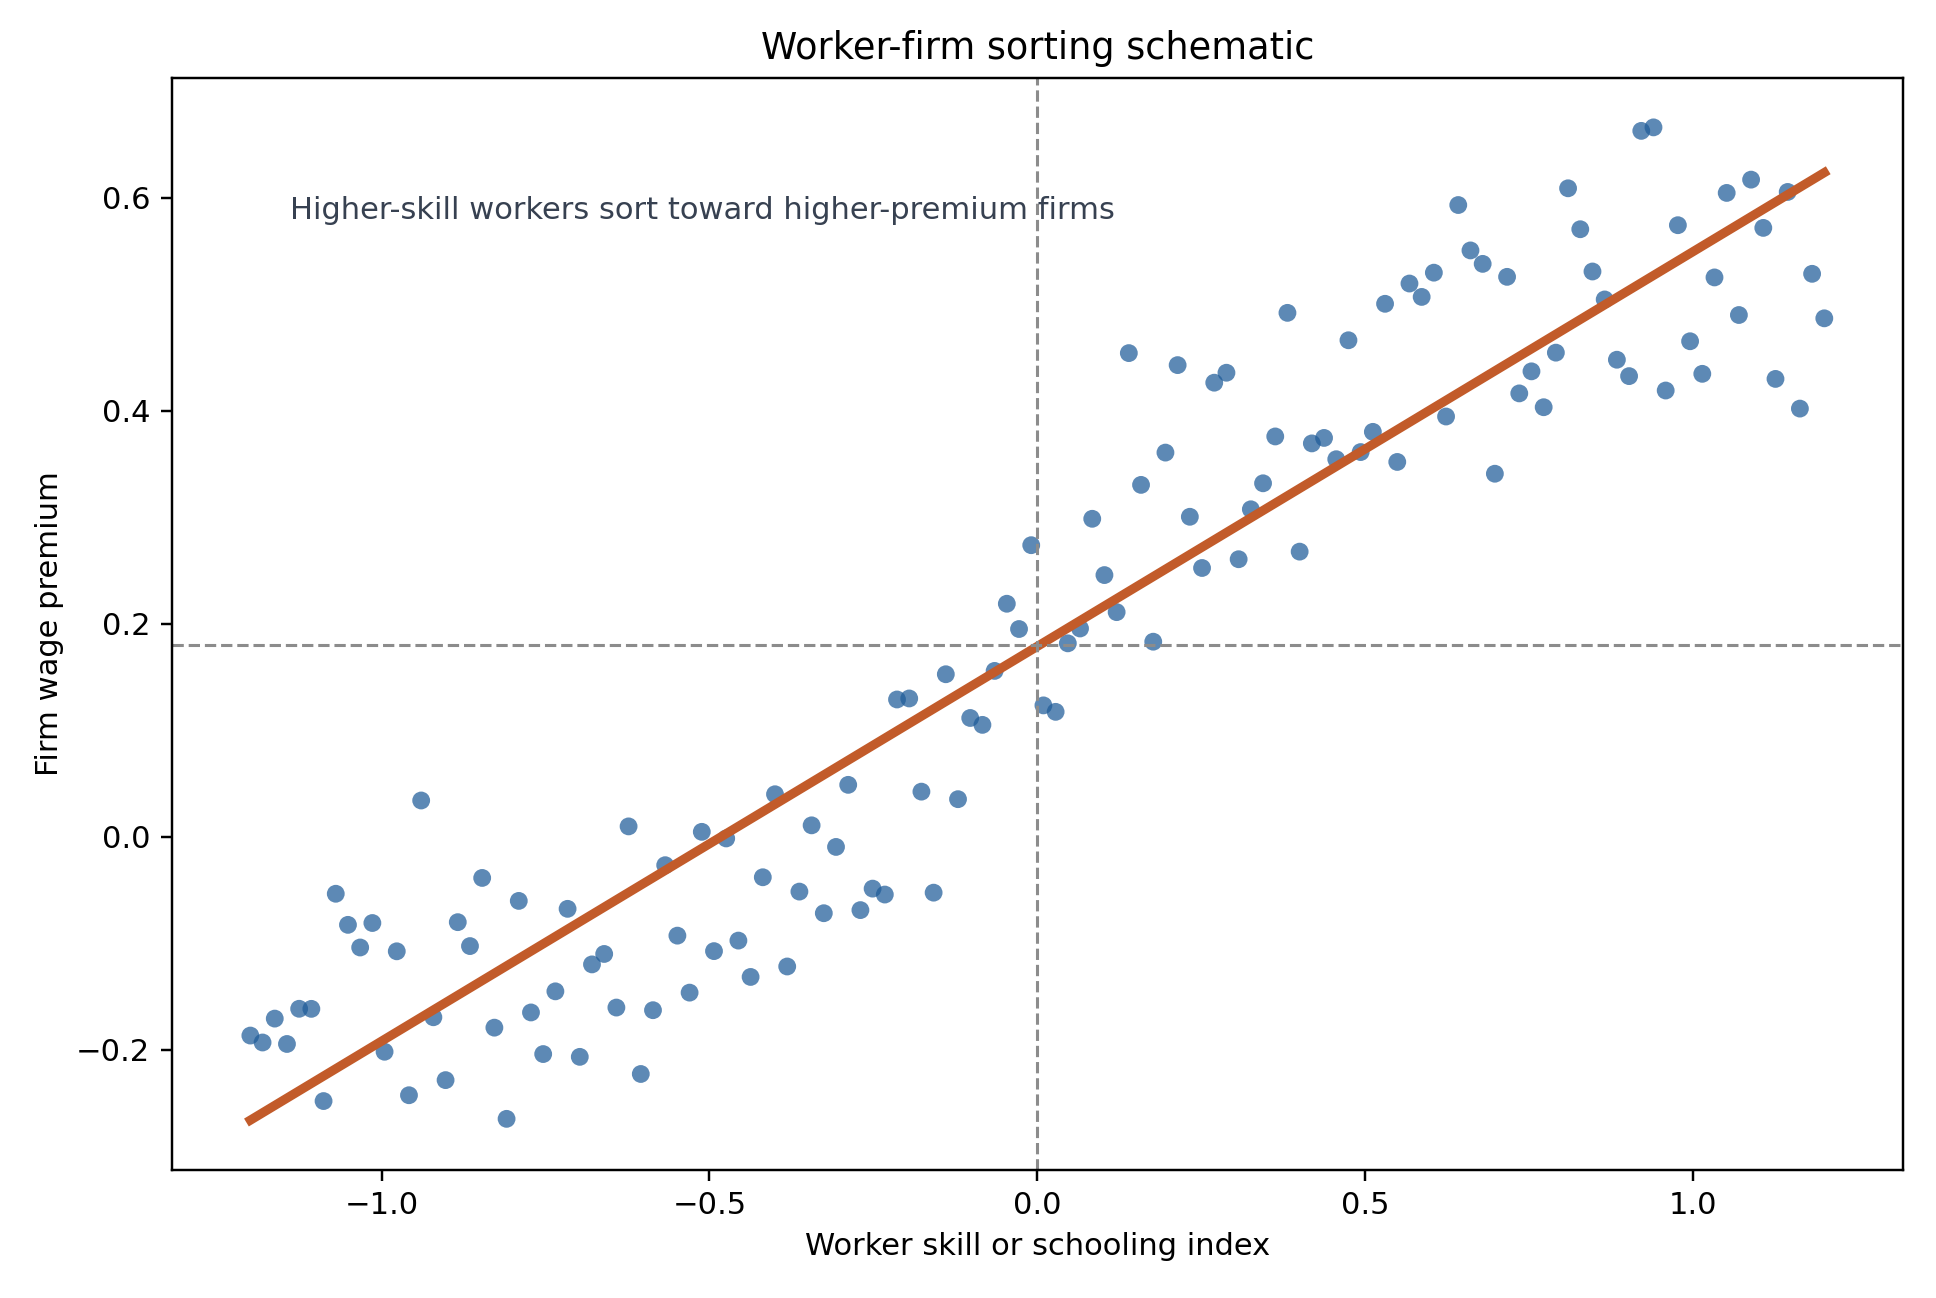
\includegraphics[height=0.72\textheight,keepaspectratio]{05-worker-firm-sorting-schematic.png}
\end{center}
\end{frame}

\begin{frame}{Design buckets and interpretation}
\begin{itemize}
    \item Descriptive wage equations: good for measurement, weak for causal interpretation.
    \item Compulsory-schooling IV: local return for the induced schooling margin.
    \item Matched worker-firm decompositions: map wage dispersion across workers and firms.
    \item Spatial sorting designs: show that some skill returns are place-mediated.
\end{itemize}
\end{frame}

\begin{frame}{Bridge to Week 6 and Week 8}
\begin{itemize}
    \item Week 6: households change schooling choices, labor supply, and observed wage offers.
    \item Week 7: amenities imply that wages are incomplete welfare objects.
    \item Week 8: inequality work needs worker, firm, and market decompositions rather than one residual ``skill premium.''
\end{itemize}
\end{frame}

\begin{frame}{Takeaways}
\begin{itemize}
    \item Mincer is a benchmark, not the truth.
    \item Changing the design changes the estimand.
    \item Returns to schooling can operate through firms and places, not only within-worker productivity.
    \item Wage determination is the discipline that connects human capital to inequality.
\end{itemize}
\end{frame}

\appendix

\begin{frame}{Appendix: optional extension block}
\begin{itemize}
    \item Worker-firm decompositions in the spirit of AKM and modern firm-inequality work.
    \item Spatial sorting and diverging city returns to skill.
    \item Optional lab reflection: how much of a schooling premium might be mediated by better firms or places?
\end{itemize}
\end{frame}

\end{document}
